\section{Nominal MPC}
 \subsection{Classical design vs MPC}
\begin{center}
\begin{tabular}{|c|c|}
     \hline
    \textbf{Classical} & \textbf{MPC} \\
    \hline
    Disturbance rejection (d$\rightarrow$ y) & Control constraints (limits)
    \\
    \hline
    Noise insensitivity (n $\rightarrow$ y & Process constraints (safety) \\
    \hline
    usually in \textbf{frequency domain} & usually in \textbf{time domain} \\ \hline
    Model uncertainty & Model \textbf{predictive} Control\\ \hline
\end{tabular}
\end{center}
predictive Control allows to \begin{itemize}
    \item include constraint in design
    \item set optimal setpoint
    \item operate plant optimal
\end{itemize}
\vfill\null\columnbreak
\subsection{MPC: Mathematical Formulation}
\begin{gather*}
    U^*_k(x(k)) := \underset{U_k}{\mathrm{argmin}}\sum^{N-1}_{i=0}I(x_{k+1},u_{k+1}) \\
    \textrm{subj. to } x_k = x(k) \textrm{ measurement} \\
    x_{k+i+1}= Ax_{k+i}+ Bu_{k+i} \textrm{ system model}
    \\
    x_{k+1} \in \mathcal{X} \textrm{ state constraints}\\
    u_{k+1} \in \mathcal{U} \textrm{ input constraints}\\
    U_k = \{u_k,u_{k+1}, \dots, u_{k+N-1}\} \textrm{ optimisation variables}
\end{gather*}
\subsection{CITOC: what we would like to solve ({\tiny Constrained finite time optimal control})}

\begin{gather*}
    J^*_\infty(x(0)) = \underset{u(\cdot)}{\mathrm{min}}\sum^\infty_{i=0}I(x_i,u_i) \\
    \mathrm{subj.\hspace{2mm} to} \hspace{3mm}x_{i+1} = Ax_i + B u_i, i = 0,\dots,\infty \\
    x_i \in \mathcal{X}, u_i \in \mathcal{U}, i = 0,\dots,\infty\\
    x_0 = x(0)
\end{gather*}

\begin{itemize}
    \item \textbf{state cost} $I(x,u)$: cost of being in state x and applying input u.
\end{itemize}
\subsection{CFTOC: what we can sometimes solve}
\begin{gather*}
    J^*_{k\rightarrow k+N|k}(x(k)) = \underset{U_k\rightarrow k+ N|k}{\mathrm{min}} \textcolor{red}{I_f(x_{k+N|k})}+ \\ \sum^{\textcolor{red}{N-1}}_{i=0}I(x_{k+i|k, u_{k+i|i}}) \\ 
    \mathrm{subj. \hspace{2mm} to \hspace{2mm}} x_{k+i+1|k}= Ax_{k+i|k} + Bu_{k+i|k} i = 0,\dots,N-1 \\
    x_{k+i|k} \in \mathcal{X}, u_{k+i|k} \in \mathcal{U}, i= 0,\dots,N-1 \\
    \textcolor{red}{x_{k+N|k} \in \mathcal{X}_f}\\
    x_{k|k} = x(k)
\end{gather*}
where $U_{k\rightarrow k + N|k}= \{u_{k|k}\dots,u_{k+N-1|k}\}$
\begin{itemize}
    \item $I_f(x_{k+N|k})$: approximates the 'tail' of the cost
    \item $\mathcal{X}_f$: Approximates the tail of the constraints 
\end{itemize}
\subsection{MPC: Mathematical Formulation}
\begin{center}
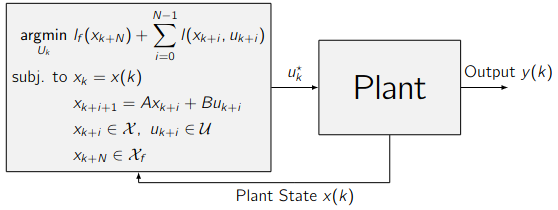
\includegraphics[width = 0.6\linewidth]{MPC_summary/Images/Screenshot from 2021-07-30 16-13-03.png}
\end{center}
\subsection{constrained Linear Optimal Control}
Cost function \[J(x_0,U) = I_f(x_N)+\sum^{N-1}_{i=0} I (x_i,u_i)\]
\begin{itemize}
    \item Squared  Euclidian norm: $I_f(x_N)=x_N^TPx_N$ and $I(x_i,u_i ) = x_i^TQx_i+u^T_iRu_i, \mathrm{with} P \succeq 0, Q\succeq 0, R\succ 0$
\end{itemize}
\subsection{Transform Quadratic Cost CFTOC $\Rightarrow$ QP}
\begin{gather*}
    J^*(x(k)) = \underset{U}{\mathrm{min}}x^T_NPx_N+ \sum^{N-1}_{i=0}x_i^TQx_i + u_j^TRu_i \\ 
    \mathrm{subj. \hspace{2mm} to \hspace{2mm}} x_{i+1}= Ax_{i} + Bu_{i} i = 0,\dotsc,N-1 \\
    x_{i} \in \mathcal{X}, u_i \in \mathcal{U}, i= 0,\dotsc,N-1 \\
    {x_{N} \in \mathcal{X}_f}\\
    x_{0} = x(k)\\
    \Downarrow\\
    \underset{z\in\mathbb{R}^n}{\mathrm{min}}\frac{1}{2}z^THz +q^Tz +r\\
    \mathrm{subj. \hspace{2mm} to\hspace{2mm} Gz\leq h}\\
    Az = b
\end{gather*}
\subsubsection{by substitution}
\begin{enumerate}
    \item \textbf{Cost:} \begin{gather*}
    J^*(x(k)) = \underset{U}{\mathrm{min}} [U^Tx(k)^T]
    \begin{bmatrix}
    H & F^T\\
    F & Y
    \end{bmatrix} [U^Tx (k)^T ]^T\\ 
    \mathrm{subj.\hspace{2mm} to\hspace{2mm}} GU \leq w + E x(k)
    \end{gather*}
    \item \textbf{Constraints:} 
\end{enumerate}
    \begin{gather*}
        \mathcal{X}= \{x|A_xx\leq b_x\}, \mathcal{X}_f = \{x|A_fx\leq b_f\}, \mathcal{U} = \{u|A_uu\leq b_u\}\\
        \Bar{A}_x =\textrm{diag}(A_x,\dotsc,A_f), \Bar{A}_u = \textrm{diag}(A_u,\dotsc), \Bar{b}_{x/u} = [b_{x/u}]^T\\ \rightarrow \Bar{A}_xX\leq \Bar{b}_x, \Bar{A}_uU\leq\Bar{b}_u
    \end{gather*}
\begin{enumerate}[resume]
    \item \textbf{Substitution}
    \begin{gather*}
        X = S^X x(k) + S^U \rightarrow \Bar{A}_x S^UU \leq \Bar{b}_x -\Bar{A}_x S^Xx(k)\\ \Rightarrow G U \leq w + E x(k)\\
      \underbrace{\begin{bmatrix}
        A_u & 0 & \dotsm & 0\\
        0 & A_u & \dotsm & 0 \\
        \vdots & \vdots & \ddots & \vdots \\
        0 & 0 & \dotsm & A_u\\ 
        0 & 0 &\dotsm & 0 \\ 
        A_xB & 0 & \dotsm & 0 \\
        A_x AB & A_x B &\dotsm & 0 \\
        \vdots & \vdots & \ddots & \vdots \\
        A_fA^{N-1}B & A_fA^{N-2}B&
        \dotsm & A_f B 
        \end{bmatrix}}_G
        \underbrace{\begin{bmatrix}
        0 \\ 0 \\ \vdots \\ 0 \\ -A_x \\ -A_x A \\ -A_xA^2\\ \vdots \\ -A_fA^N
        \end{bmatrix}}_E \underbrace{\begin{bmatrix}
        b_u \\ b_u \\ \vdots \\ b_u \\ b_x \\ b_x \\ b_x\\ \vdots \\b_f
        \end{bmatrix}}_W
    \end{gather*}
\end{enumerate}
$\rightarrow$ For a given $x_k$, solution $U^*$ can be found with a QP solver. 
\subsubsection{Construction of the QP without Substitution}
\begin{enumerate}
    \item \textbf{Cost:}\begin{gather*}
        J^*(x_k) =  \underset{z}{\textrm{min}}\begin{bmatrix}
        z^T & x_k^T
        \end{bmatrix} \begin{bmatrix}
        \Bar{H} & 0 \\ 0& Q
        \end{bmatrix} \begin{bmatrix}
        z^T & x_k^T
        \end{bmatrix}^T\\ \textrm{subj. to: } G_{in}z \leq W_{in} + E_{in}x_k\\
        G_{eq}z = E_{eq}x_k \textrm{with} z = [x_1^T, \dotsc, x_N^T, u_0^T, \dotsc, u_{N-1}^T],\\\Bar{H} = \textrm{diag}(Q,\dotsc,Q,P,R,\dotsc, R)
    \end{gather*}
        \item \textbf{Equalities} \begin{gather*}
            x_{i+1} = Ax_i+Bu_i:\\
            G_{eq} = \begin{bmatrix}
            \begin{array}{@{}ccc|ccc@{}}
            I & & &-B & & \\
            -A & \ddots & & &\ddots & \\
            & -A & I & & &-B 
            \end{array}
            \end{bmatrix}, E_{qe} = \begin{bmatrix}
            A\\ 0\\ \vdots
            \end{bmatrix}
        \end{gather*}
    \item \textbf{Inequalities: }with $\mathcal{X} = \{x|A_x x\leq b_x\},\\ \mathcal{X}_f = \{x|A_fx\leq b_f\}, \mathcal{U}= \{u|A_u u \leq b_u\}$\\ 
    and $\Bar{A}_x,\Bar{A}_u,\Bar{b}_x,\Bar{b}_u $ from above 
    \begin{gather*}
        G_in = \begin{bmatrix}
        0 & & \\ 
        & \Bar{A}_x & \\
        & & \Bar{A}_u
        \end{bmatrix}, w_{in} = \begin{bmatrix}
            \Bar{b}_x\\ \Bar{b}_u
        \end{bmatrix}, E_{in} = \begin{bmatrix}
        -A_x \\ 0
        \end{bmatrix}
    \end{gather*}
\end{enumerate}
\subsubsection{Quadratic Cost State Feedback Solution}
\begin{gather*}
J^*(x_k) = \underset{U}{\textrm{min}} 
    \begin{bmatrix}
    U^T & x_k^T
    \end{bmatrix} \begin{bmatrix}
    H & F^T \\ F & Y
    \end{bmatrix} \begin{bmatrix}
    U^T & x_k^T
    \end{bmatrix}^T \\ 
    \textrm{subj. to } GU \leq w + E x_k \end{gather*}
    is a multiparametric quadratic program with the \textbf{solution properties: } \begin{itemize}
        \item First component of the solution: $u_0^* = \kappa(x_k) \forall x_k \in \mathcal{X}_0$ where $\kappa: \mathbb{R}^n \rightarrow\mathbb{R}^m$ is continuous and piecewise affine on Polyhedra: \[\kappa(x) = F^jx+g^j \textrm{ if }x\in CR^j  1, \dotsc, N^r\]
        \item Polyhederal sets $CR^j = j= \{x\in \mathbb{R}^n|H^jx\leq K^j, j = 1, \dotsc, N^r\}$ are partition of the feasible polyhedron $\mathcal{X}_0$
        \item The value function $J^*(\mathcal{X}_k$ is convex and piecewise quadratic on polyhedra
    \end{itemize}
\subsection{Transformation: P-Norm Cost CFTOP $\Rightarrow LP$}
\subsubsection{$\ell_\infty$ minimization}
\begin{gather*}
    \underset{x\in\mathbb{R}^n}{\textrm{min}}||x||_\infty = \underset{x\in \mathbb{R}^n}{\textrm{min}}[\textrm{max}\{x_1,\dotsc,x_n, -x_1,\dotsc, -x_n\}] \\ \textrm{subj to. } Fx \leq g \\
    \Leftrightarrow \underset{x,t}{\textrm{min }} t \textrm{ subj. to:} x_i\leq t , -x_i \leq t \Leftrightarrow -\mathbf{1}_nt \leq \mathbf{1}_n t \textrm{ and } Fx \leq g 
\end{gather*}
\subsubsection{$\ell_1$ minimization}
\begin{gather*}
    \underset{x \in \mathbb{R}^n}{\textrm{min }}||x||_1=\underset{x \in \mathbb{R}^n}{\textrm{min }}[\sum^m_{i=1}\textrm{max }\{x_i, -x_i\}]\\ \textrm{subj. to } -t \leq x \leq t \textrm{ and } F x \leq g\\ 
    \Leftrightarrow \underset{x,t}{\textrm{min}} \sum ^m_{i = 1} t_i \textrm{subj. to: } x_i \leq t , -x_i \leq t \Leftrightarrow \underset{x,t}{\textrm{min }} \mathbf{1}_n t\\ \textrm{subj. to: } -t \leq x \leq t \textrm{ and } Fx \leq g
\end{gather*}
\vfill\null\columnbreak
\subsubsection{Construction of LP with Substitution ($\infty-$Norm)}
\begin{enumerate}
    \item \textbf{Cost: } $\underset{z}{\textrm{min }}\epsilon_N^x+ \sum ^{N-1}_{i=0} \epsilon_i^x +\epsilon_i^u$ subj. to: $\pm Qx_i \leq \mathbf{1} \epsilon_i^x, \pm P x_N \leq \mathbf{1} \epsilon^x_N, \pm Rx_i \leq \mathbf{1}\epsilon_i^u$
    \item \textbf{Substitution:} $x_i = S_i^xx(k) + S_i^u U \rightarrow -\mathbf{1} \epsilon_i^x \leq \pm Qx_i, -\mathbf{1}\epsilon_N^x \leq \pm Px_N, -\mathbf{1}\epsilon_i^u\leq \pm Ru_i$\begin{gather*}\Rightarrow \underset{z}{\textrm{min }}c^Tz \textrm{ subj. to:} \Bar{G}z \ \leq \Bar{w}+\Bar{S}x_k, \\\Bar{G}= \begin{bmatrix}
    G_\epsilon & G_U\\
    0 & G
    \end{bmatrix}, \Bar{S}=\begin{bmatrix}
    S_\epsilon \\ S_U
    \end{bmatrix}, \Bar{w}= \begin{bmatrix}
    w_\epsilon \\ w_U
    \end{bmatrix}
    \end{gather*}
\end{enumerate}
$z := \{\epsilon_0^x,\dotsc,\epsilon_N^x,\epsilon_0^u,\dotsc,\epsilon^u_{N-1}, u_0^T, \dotsc,u_{N-1}^T\} \in \mathbb{R}^s \rightarrow $ for $x_k, U^*$ obtained via LP solver 
\subsubsection{1-/$\infty$- Norm State Feedback Solution}
$\underset{z}{\textrm{min }} c^Tz$ subj. to: $\Bar{G}z \leq \Bar{w}+\Bar{S}x_k$ is a multiparam. lin. program
\begin{itemize}
    \item First component of solution: $u_0^* = \kappa(x_0) \forall x_0 \in \mathcal{X}_0 $ \textbf{Else, the same as mp-qp}
    \item The value function $J^*(x_0)$ is convex and piecewise linear on polyhedra
\end{itemize}
    
\subsection{Stability of MPC}
\textbf{3 assumptions}
\begin{enumerate}
    \item Stage cost is positive definite, i.e. it is strictly positive and only zero at the origin
    \[Q \textrm{ and } R \succ 0\]
    \item Terminal set is \textbf{invariant} under the local control law $\mathcal{K}_f(x_i)$:\[x_{i+1} = Ax_i+B\mathcal{K}_f(x_i), \hspace{3mm} \forall x_i \in \mathcal{X}_f\]
    All state and input \textbf{constraints are satisfied} in $\mathcal{X}_f$:
    \[\mathcal{X}_f \subseteq \mathcal{X}, \mathcal{K}_f (x_i) \in \mathcal{U} \hspace{3mm} \forall x_i \in \mathcal{X}_f\]
    \item Terminal cost is a continous \textbf{Lyapunov function} in the terminal set $\mathcal{X}_f$ and satisfies \[I_f(x_{i+1}) - I_f(x_i) \leq -I(x_i,\mathcal{K}_f(x_i)), \hspace{3mm} \forall x_i \in \mathcal{X}_f\]
\end{enumerate}
\section{Invariance}
Region s.th autonomous system satisfies constraints for all time 
\subsubsection{Positive Invariance Set}\fbox{\parbox{0.97\linewidth}{
A set $\mathcal{O}$ is said to be a positive invariant set for the autonomous system if $x_k \in \mathcal{O} \Rightarrow x_{k+1} \in \mathcal{O} \forall k \in\{0,1,\dots\}$}}
if the invariant set is within the constraints, it provides a set of initial states from which the trajectory will never violate the system constraints
\subsubsection{Pre Set}
\fbox{\parbox{0.97\linewidth}{Given a set $\mathcal{S} $ and the system $x_{k+1} = g(x_k),$ the pre-set of $\mathcal{S}$ is the set of states that evolve into the target set $\mathcal{S}$ in one time step: pre$(\mathcal{S}) := \{x|g(x)\in \mathcal{S}\}$ if $\mathcal{S}:= \{x|Fx\leq f\}$, then pre($\mathcal{S})=\{x|FAx\leq f\}$ for $x_{k+1} =a x_k$}}
\subsubsection{Invariant Set Conditions}
\begin{itemize}
    \item A set $\mathcal{O}$ is a positive invariant set iff $\mathcal{O} \subseteq$ pre$(\mathcal{O}$)
    \item\textbf{Necessary:} if $\mathcal{O} \nsubseteq \textrm{pre}(\mathcal{O}),$ then $\exists \Bar{x} \in \mathcal{O}$ s.th. $\Bar{x} \notin$ pre$(\mathcal{O})$. From tge definition of pre($\mathcal{O}$), $g(\Bar{x}) \notin \mathcal{O}$ and thus $\mathcal{O}$ is \textbf{not} a PIS.
    \item\textbf{Sufficient:} if $\mathcal{O}$ is not a PIS, then $\exists \Bar{x} \in \mathcal{O}$ s.th. $g(\Bar{x}) \notin\mathcal{O}$ this implies that $\Bar{x} \in \mathcal{O}$ and $\Bar{x} \notin$ pre($\mathcal{O}$) and thus $\mathcal{O} \nsubseteq$ pre$(\mathcal{O})$
\end{itemize}